\documentclass{article}
\usepackage[utf8]{vietnam}
\usepackage{graphicx}
\usepackage{setspace}
\usepackage{fancyhdr}
\usepackage{pifont}
\usepackage{tikz}
\usepackage{tocloft}   % For \addcontentsline
\usepackage[left=3cm,right=2cm,top=2cm,bottom=2cm]{geometry}
\graphicspath{ {./images/} }
\makeatletter
\renewcommand{\tableofcontents}{%
	\@starttoc{toc}%
}
\makeatother
\begin{document}
%------------------------------------------------------------
%|						COVER PAGE						
%------------------------------------------------------------
% Vẽ khung cho trang đầu tiên

\begin{center}
	\pagenumbering{gobble}
	\fontsize{16}{20}\selectfont
	\textbf{TRƯỜNG ĐẠI HỌC CÔNG THƯƠNG TP.HỒ CHÍ MINH\\ 
		\textbf{KHOA CÔNG NGHỆ THÔNG TIN}}
	
	\vspace{0.8cm}
	\begin{figure}[htp]
		\begin{center}
			\includegraphics[scale=0.08]{images/logo.png}
		\end{center}
	\end{figure}
	\vspace{1cm}
	\fontsize{24}{20}\selectfont\textbf{BÁO CÁO THỰC TẬP TỐT NGHIỆP\\}
	
	\vspace{3cm}
	\fontsize{24}{20}\selectfont\textbf{ỨNG DỤNG YOLO VÀ OPENCV THIẾT KẾ HỆ THỐNG PHÁT HIỆN CON NGƯỜI VÀ ĐÁNH GIÁ AN TOÀN}
\end{center}
\vspace{2cm}
\begin{center}
	\fontsize{14}{20}\selectfont\textit{}{Sinh viên thực hiện: HOÀNG THẾ ANH}\\
	\fontsize{14}{20}\selectfont\textit{}{Mã sinh viên: 2001202008 Lớp: 11DHTH9}

\end{center}
\pagebreak	
%------------------------------------------------------------
%|						COVER PAGE						
%------------------------------------------------------------
% Vẽ khung cho trang đầu tiên

\begin{center}
	\pagenumbering{gobble}
	\fontsize{16}{20}\selectfont
	\textbf{TRƯỜNG ĐẠI HỌC CÔNG THƯƠNG TP.HỒ CHÍ MINH\\ 
		\textbf{KHOA CÔNG NGHỆ THÔNG TIN}}
	
	\vspace{0.8cm}
	\begin{figure}[htp]
		\begin{center}
			\includegraphics[scale=0.08]{images/logo.png}
		\end{center}
	\end{figure}
	\vspace{1cm}
	\fontsize{24}{20}\selectfont\textbf{BÁO CÁO THỰC TẬP TỐT NGHIỆP\\}
	
	\vspace{3cm}
	\fontsize{24}{20}\selectfont\textbf{ỨNG DỤNG YOLO VÀ OPENCV THIẾT KẾ HỆ THỐNG PHÁT HIỆN CON NGƯỜI VÀ ĐÁNH GIÁ AN TOÀN}
\end{center}
\vspace{2cm}
\begin{center}
	\fontsize{14}{20}\selectfont\textit{}{Sinh viên thực hiện: HOÀNG THẾ ANH}\\
	\fontsize{14}{20}\selectfont\textit{}{Mã sinh viên: 2001202008 Lớp: 11DHTH9}

\end{center}
\pagebreak
	%------------------------------------------------------------
	%|					CAM ĐOAN PAGE					|
	%------------------------------------------------------------
    \pagestyle{fancy}
	\fancyhf{}
	\chead{\thepage}
	\renewcommand{\headrulewidth}{0pt}
	\begin{center}
		\pagenumbering{roman}\setcounter{page}{1}
		\fontsize{16}{20}\selectfont
		\textbf{LỜI CAM ĐOAN\\} 
	\end{center}
	\setstretch{1.5}
	\fontsize{13}{13}\selectfont
	\paragraph{}
	Tôi xin cam đoan đây là công trình nghiên cứu của riêng tôi. Các số liệu, kết quả nêu trong Báo cáo thực tập tốt nghiệp là trung thực và chưa từng được ai công bố trong bất kỳ công trình nào khác.
	\paragraph{}
    	Tôi xin cam đoan rằng mọi sự giúp đỡ cho việc thực hiện Báo cáo thực tập tốt nghiệp này 
    đã được cảm ơn và các thông tin trích dẫn trong Báo cáo thực tập tốt nghiệp đã được chỉ rõ nguồn gốc.
	
	\begin{flushright}
            \textbf {Sinh viên thực hiện báo cáo} \\
            \textit{(Ký và ghi rõ họ tên)}
        \end{flushright}
	\pagebreak	
	%------------------------------------------------------------
	%|					ACKNOWLEDGEMENT PAGE					|
	%------------------------------------------------------------
	\pagestyle{fancy}
	\fancyhf{}
	\chead{\thepage}
	\renewcommand{\headrulewidth}{0pt}
	\begin{center}
		\pagenumbering{roman}\setcounter{page}{1}
		\fontsize{16}{20}\selectfont
		\textbf{LỜI CẢM ƠN\\} 
	\end{center}
	\setstretch{1.5}
	\fontsize{13}{13}\selectfont
	\paragraph{}
	Trong thời gian thực tập tại công ty TNHH LUNA NEXUS VN INC., em xin cảm ơn quý công ty đã tạo điều kiện để em có thể hoàn thành được kì thực tập của mình.
	\paragraph{}
	Xin cảm ơn Kĩ sư Trần Minh Vương, anh là người trực tiếp giám sát quá trình thực tập cũng như là người hỗ trợ em tìm kiếm tài liệu chuyên ngành và giải đáp các thắc mắc về dự án thực tập trong suốt quá trình làm việc tại công ty.

	\paragraph{}
	Em xin chân thành cảm ơn Trường Đại học Công Thương Thành phố Hồ Chí Minh đã tạo điều kiện để em có thể được trực tiếp học tập ở doanh nghiệp và thu được nhiều bài học cũng như là kinh nghiệm quý báu trong quá trình làm việc.
	\paragraph{}
	Cảm ơn gia đình, những người bạn học đã luôn cổ vũ mình và tạo điều kiện giúp cho mình có thể hoàn thành tốt được dự án thực tập tại học kì doanh nghiệp.
	\paragraph{}
	Em xin cảm ơn.
	\pagebreak	

	%------------------------------------------------------------
	%|					TABLEOFCONTENT PAGE						|
	%------------------------------------------------------------
	\begin{center}
		\pagenumbering{arabic}\setcounter{page}{1}
		\fontsize{16}{20}\selectfont
		\textbf{MỤC LỤC\\} 
		
	\end{center}
	\setstretch{1.5}
	\fontsize{13}{13}\selectfont
	\tableofcontents
	\addcontentsline{toc}{section}{LỜI CẢM ƠN}
	
	
	
	
	
	\pagebreak
	%------------------------------------------------------------
	%|					CHAPTER 1		                     	|  
	%| GIỚI THIỆU CHUNG ĐƠN VỊ THỰC TẬP              			|
	%------------------------------------------------------------
	\begin{center}
		\pagenumbering{arabic}\setcounter{page}{2}
	\end{center}
	
	\begin{flushleft}
		
		\fontsize{16}{20}\selectfont
		\section*{CHƯƠNG 1: GIỚI THIỆU CHUNG ĐƠN VỊ THỰC TẬP }
		\addcontentsline{toc}{section}{CHƯƠNG 1: GIỚI THIỆU CHUNG ĐƠN VỊ THỰC TẬP }
		\fontsize{13}{13}\selectfont
		%
		% Phần 1
		%
        \setcounter{section}{1}


        \subsection{Thông tin về đơn vị thực tập}
		\subsubsection{Sơ lược về sự hình thành và phát triển của đơn vị}
		\subsubsection{Tổ chức và các lĩnh vực hoạt động của đơn vị}
		\subsubsection{Tổ chức quản lý sử dụng các nguồn lực của đơn vị}
		\subsubsection{Cơ cấu tổ chức}
		\subsubsection{Tình hình hoạt động kinh doanh của doanh nghiệp}

		\subsection{Thông tin về vị trí sinh viên tham gia thực tập}
		\subsubsection{Giới thiệu chung về vị trí công tác}
		\subsubsection{Đặc điểm, yêu cầu}
		\subsubsection{Cơ cấu tổ chức, nhiệm vụ liên quan}
	%------------------------------------------------------------
	%|					CHAPTER 2		                     	|  
	%| PHÂN TÍCH THỰC TRẠNG CỦA VẤN ĐỀ CÓ LIÊN QUAN ĐẾN
    %| ĐỀ TÀI MÀ SINH VIÊN CHỌN VIẾT BÁO CÁO THỰC TẬP TẠI DOANH NGHIỆP THỰC TẬP             			|
	%------------------------------------------------------------
	\pagestyle{fancy}
	\fancyhf{}
	\fancyfoot[R]{\thepage}
\begin{flushleft}
    \fontsize{16}{20}\selectfont
    \section*{CHƯƠNG 2: PHÂN TÍCH THỰC TRẠNG CỦA VẤN ĐỀ CÓ LIÊN QUAN ĐẾN
    ĐỀ TÀI MÀ SINH VIÊN CHỌN VIẾT BÁO CÁO THỰC TẬP TẠI DOANH NGHIỆP THỰC TẬP}
    \addcontentsline{toc}{section}{CHƯƠNG 2: PHÂN TÍCH THỰC TRẠNG CỦA VẤN ĐỀ CÓ LIÊN QUAN ĐẾN
    ĐỀ TÀI MÀ SINH VIÊN CHỌN VIẾT BÁO CÁO THỰC TẬP TẠI DOANH NGHIỆP THỰC TẬP}
    \fontsize{13}{20}\selectfont
    \paragraph{}
    \fontsize{13}{20}\selectfont Trong quá trình thực tập tại công ty, em đã được giao dự án về phát triển phần mềm sử dụng YOLO và OpenCV để xác định và đưa ra cảnh báo đối với các đối tượng là con người trong một khu vực cụ thể.\\
    \setcounter{section}{2}
    \setcounter{subsection}{0}
    
    \subsection{Giải Pháp}
    \fontsize{13}{13}\selectfont\paragraph{}
    Để giải quyết các vấn đề trên, mô hình nhận diện đối tượng YOLO và bộ OpenCV được úng dụng vào giải pháp theo dõi con người và đánh giá an toàn. \\
    
    \subsection{Phân tích đánh giá tình hình thực tế theo chủ đề thực tập tại đơn vị}
    \subsubsection{Vấn Đề Đặt Ra}
    \fontsize{13}{20}\selectfont Vấn đề được đặt ra là phải làm sao để có thể xác định được chủ thể con người trong camera (Camera an ninh, điện thoại,...) và xác nhận xem chủ thể có ở trong khu vực được đánh dấu là an toàn hay không, vấn đề này có thể được áp dụng vào các tình huống trong đời sống hàng ngày cũng như trong doanh nghiệp, sản xuất:\\ 
    \begin{itemize}
        \item Trong gia đình: \\
        Bài toán này có thể giúp phụ huynh có thể trông con em mình, ví dụ như thông qua camera giám sát và các điểm thiết lập đã được cài đặt sẵn,phụ huynh có thể giám sát được xem là trẻ có đang trong khu vực an toàn hay không,...
        \begin{figure}[htbp]
            \centering
            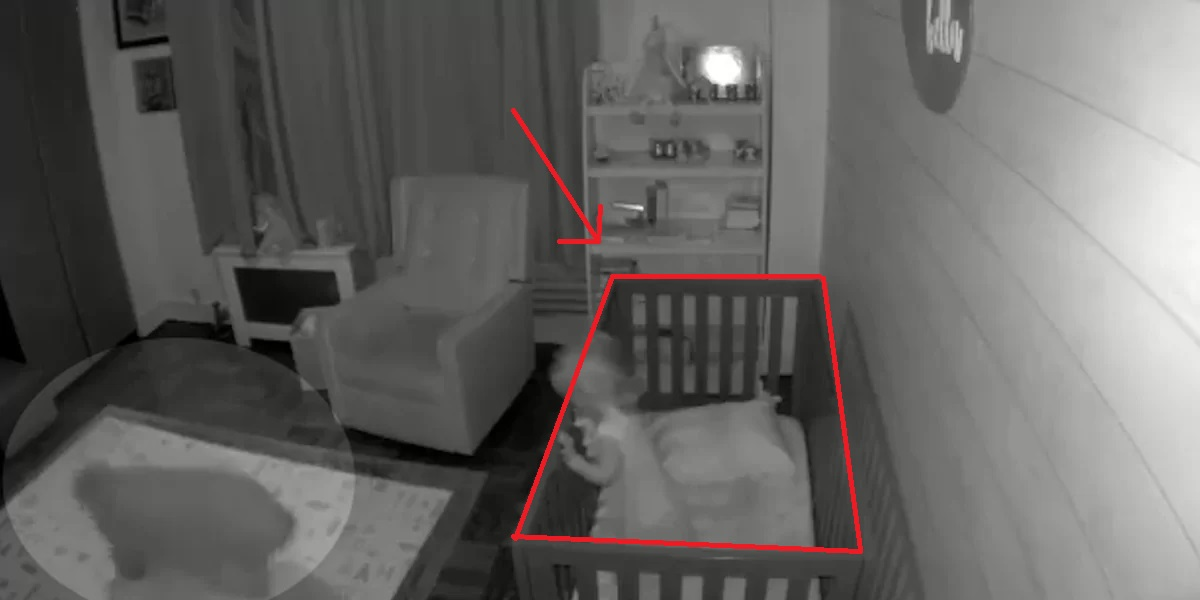
\includegraphics[width=0.5\textwidth]{images/TH1.jpg}
            \caption{Trong trường hợp gia đình.}
            \label{fig:img_1_GD}
        \end{figure}
        \item Trong văn phòng:\\
        Trong văn phòng, có thể giám sát xem, nhân viên có đang làm việc trong khu vực chỉ định hay không,...
        \begin{figure}[htbp]
            \centering
            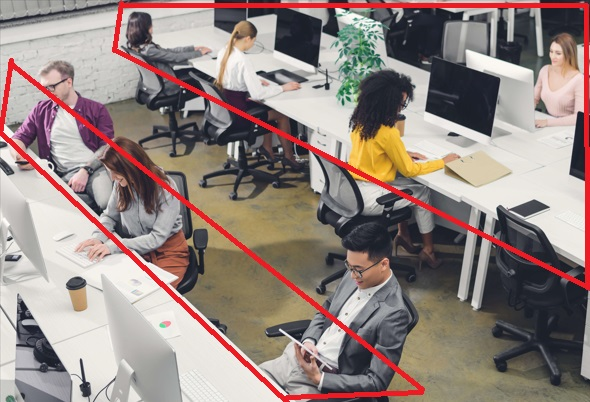
\includegraphics[width=0.5\textwidth]{images/TH2.jpg}
            \caption{Trong trường hợp văn phòng.}
            \label{fig:img_2_VP}
        \end{figure}
        \item Trong sản xuất:\\
        Trong sản xuất, việc các công nhân có làm đúng được vị trí của mình được phân công hay không,...
        \begin{figure}[htbp]
            \centering
            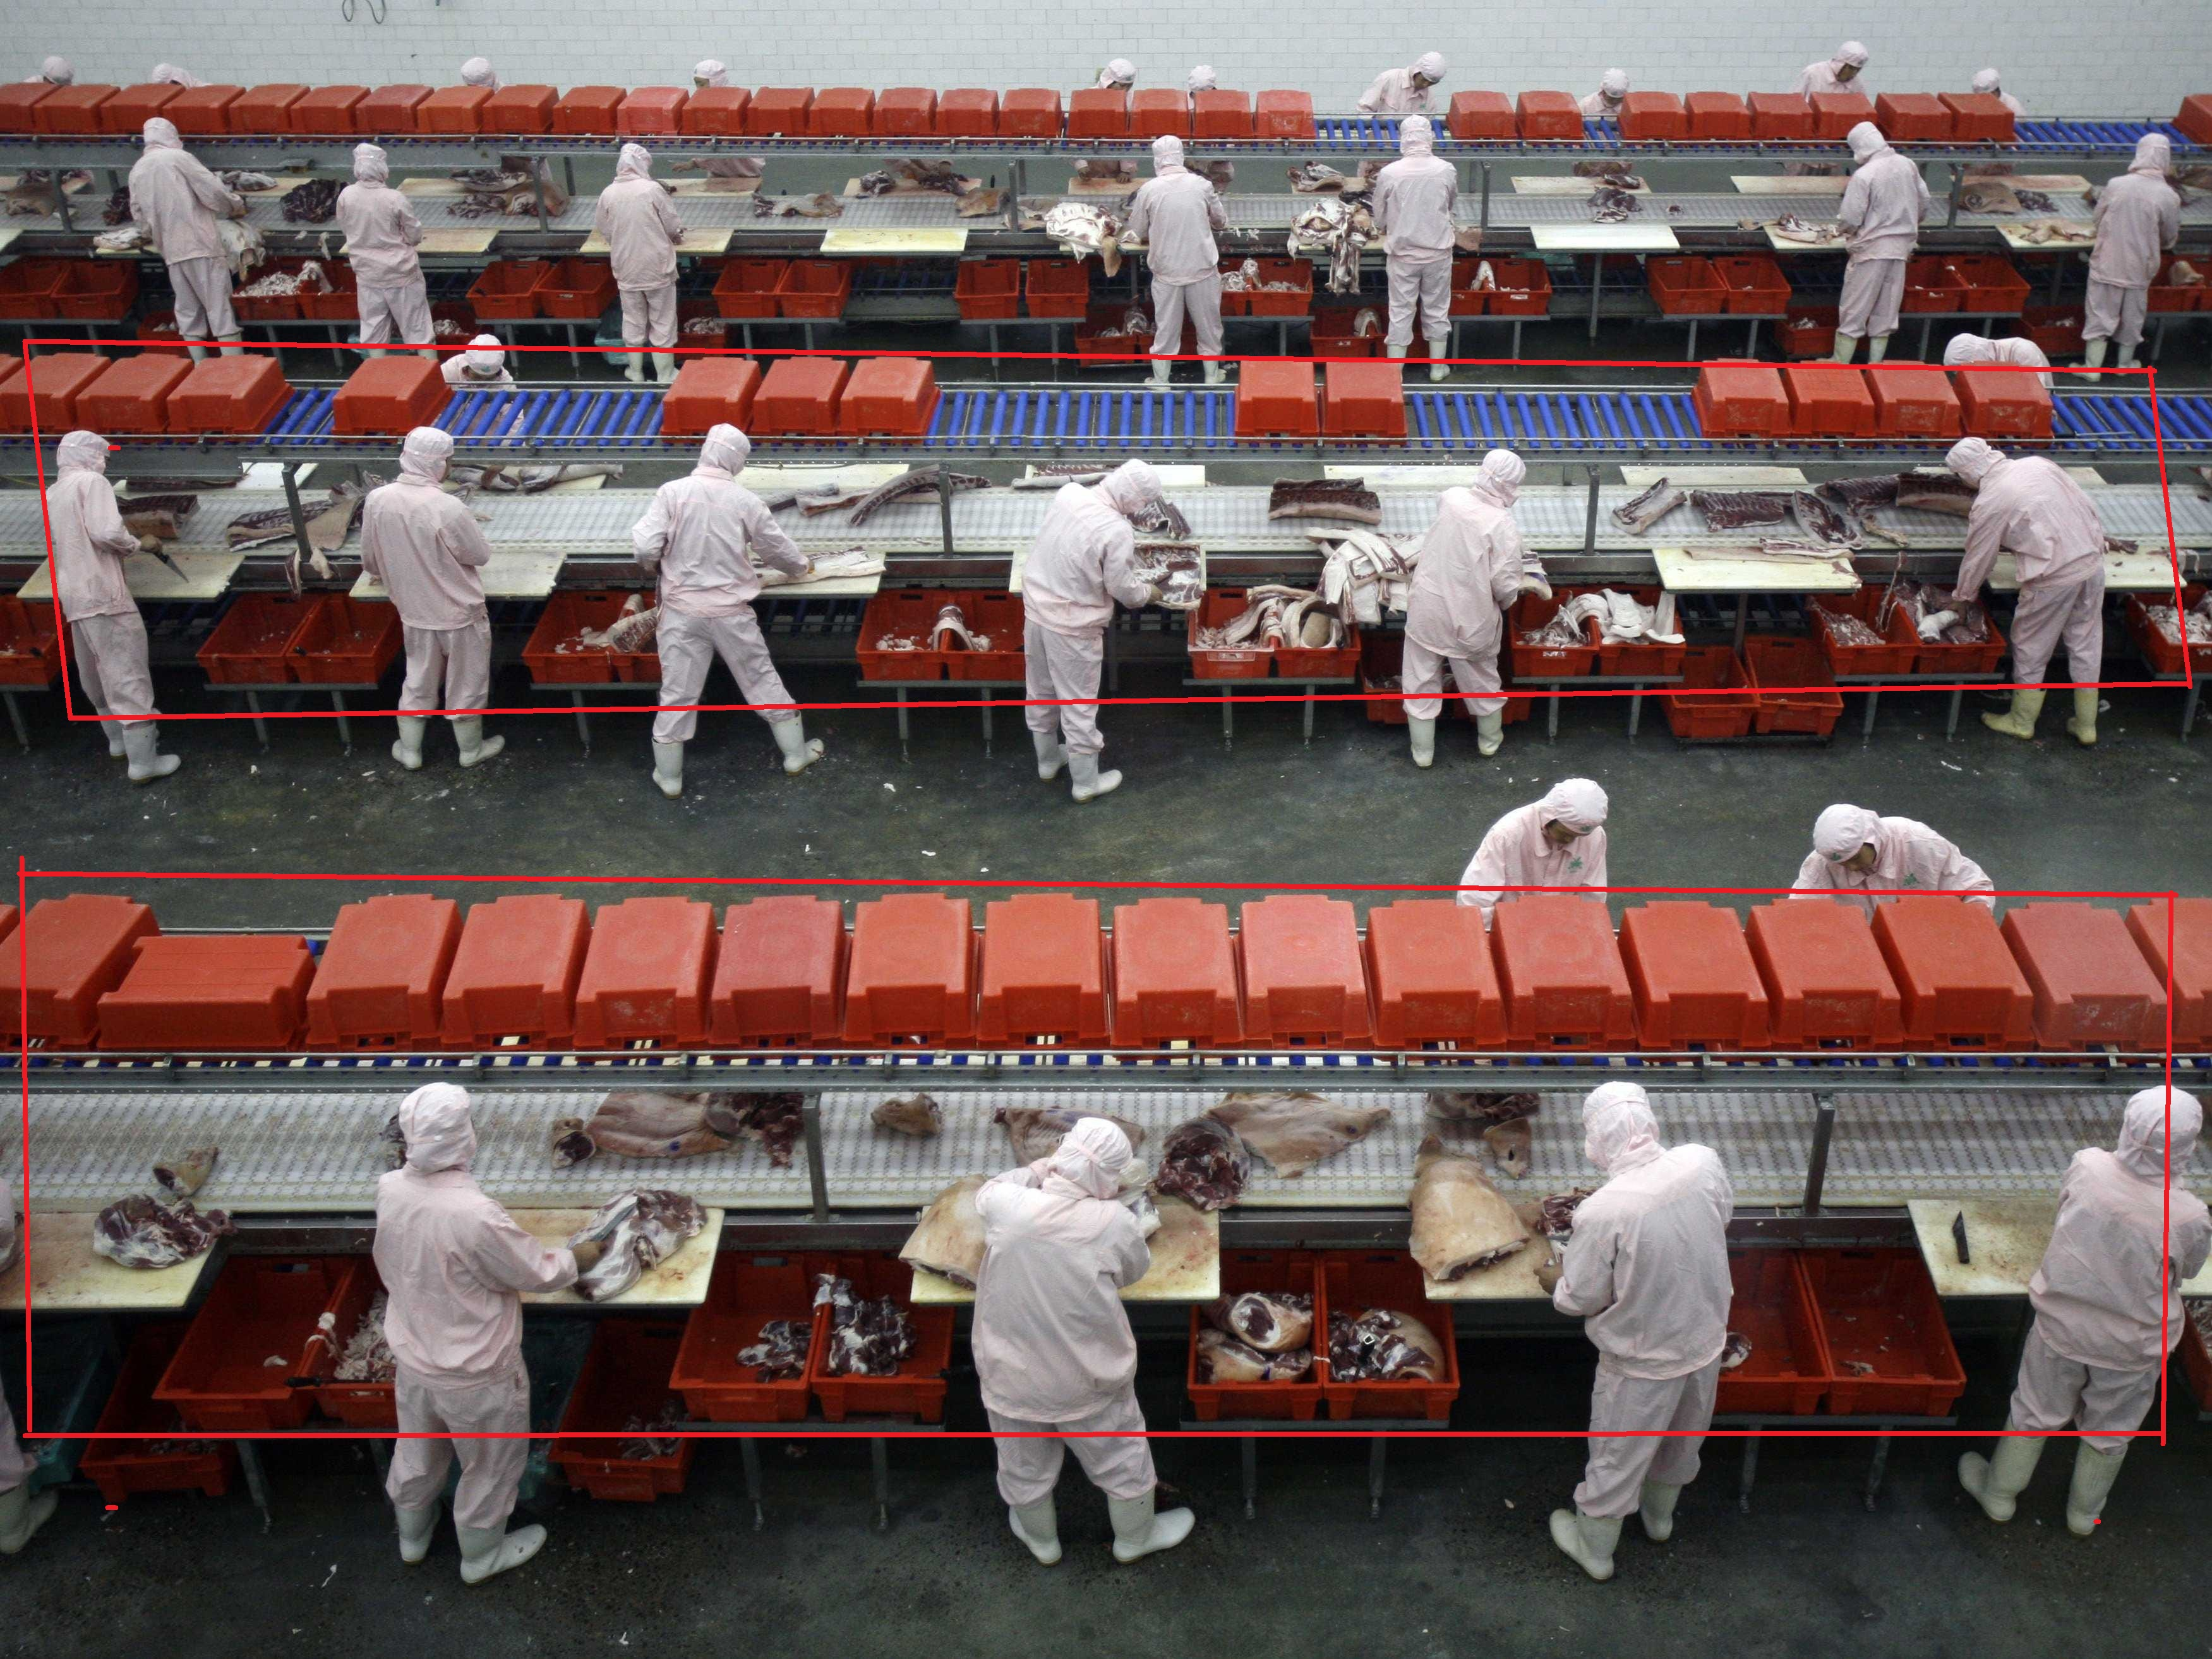
\includegraphics[width=0.5\textwidth]{images/TH3.jpg}
            \caption{Trong trường hợp xí nghiệp.}
            \label{fig:img_3_XN}
        \end{figure}
    \end{itemize}
    

    
    \subsection{Ưu điểm, hạn chế của vấn đề phân tích nêu trên}
    \subsection{Tiến độ thực hiện công việc}
    \subsection{Sơ lược các kỹ thuật, công nghệ liên quan đến các nội dung đã trình bày}
\end{flushleft}
	
		\fontsize{14}{20}\selectfont
		
		\section*{CHƯƠNG 3: PHÂN TÍCH HỆ THỐNG}
		\addcontentsline{toc}{section}{CHƯƠNG 3: PHÂN TÍCH HỆ THỐNG}
		\fontsize{14}{20}\selectfont
		\setcounter{section}{3}
		\subsection{ Mô hình use case }
	
		
		\fontsize{14}{20}\selectfont
		\subsubsection{Use case đăng nhập}
		\fontsize{13}{13}\selectfont

		\begin{table}[h!]
		\centering
			\begin{tabular}{|l|l|}
				\hline
				Tên Use case            & UC Đăng nhập\\ \hline
				Tác nhân:            & Lễ tân, quản lý, kế toán \\ \hline
				Kích hoạt     &Người dùng nhấn nút đăng nhập \\ \hline
		    	Mô tả   & Use case này mô tả quy trình đăng nhập vào hệ thống. \\ \hline
				Điều kiện tiên qyết       & Là nhân viên thuộc quản lý của khách sạn.\\& Đã được cấp mã số và mật khẩu có trong CSDL.\\ & Thiết bị dùng để đăng nhập có kết nối vào mạng nôi bộ.\\ \hline
				Flow of event        & \begin{tabular}[c]{@{}l@{}}Actors:\\ Người dùng nhập thông tin đăng nhập gồm mã số và mật khẩu đã được cấp từ trước và nhấn vào nút “Đăng nhập”.\\  System:\\ Nếu thiết bị có kết nối vào mạng nội bộ, hệ thống thực hiện thao tác kiểm tra mã số và mật khẩu nhận được từ giao diện người dùng. Nếu kiểm tra mã số và mật khẩu trùng khớp với CSDL, hệ thống sẽ chuyển sang trang làm việc theo đúng phân quyền của người dùng đó.\end{tabular} \\ \hline
				Luồng thay thế       & Thiết bị đăng nhập không kết nối vào mạng nội bộ.\\&Người dùng để trống một trong hai ô mã số hoặc mật khẩu và ấn đăng nhập, hệ thống hiển thị thông báo yêu cầu nhập đủ thông tin đăng nhập. Nếu quá số lần quy định hệ thống tự ngắt kết nối với thiết bị đó.\\&Người dùng để trống cả mã số và mật khẩu đăng nhập và ấn đăng nhập, hệ thống hiển thị thông báo yêu cầu nhập đủ thông tin đăng nhập. Nếu quá số lần quy định hệ thống từ ngắt kết nối với thiết bị đó.\\.\\&Người dùng nhập đủ cả 2 ô nhưng nhập sai một trong hai ô mã số hoặc mật khẩu, hệ thống hiển thị thông báo yêu cầu nhập lại ô bị sai so với CSDL. Nếu quá số lần quy định hệ thống tự khóa tài khoản đó và ngắt kết nối với thiết bị dùng để đăng nhập đó.\\ \hline
				Điều kiện sau \\ &Hiển thị thông báo đăng nhập thành công và chuyển đến trang làm việc đúng theo phân quyền của nhân viên vừa đăng nhập.\\ \hline
				Điều kiện thoát       & Người dùng đăng nhập thành công và hệ thống chuyển qua trang làm việc theo đúng phân quyền của người dùng đó.\\&Người dùng không thực hiện theo thông báo nhập thông tin đầy đủ quá số lần quy định và bị ngắt kết nối vào mạng nội bộ.\\ &Người dùng không thực hiện theo thông báo nhập sai thông tin quá số lần quy định và bị ngắt kết nối vào mạng nội bộ.\\ &Thiết bị dùng để đăng nhập không có kết nối vào mạng nội bộ..\\ \hline
			\end{tabular}
			\caption{Usecase đăng nhập}
			\label{table}
		\end{table} 
		\pagebreak
		
		\subsubsection{Use case lập hóa đơn đặt phòng}
		
			\begin{table}[h!]
		\centering
			\begin{tabular}{|l|l|}
				\hline
				Tên Use case            & Lập hóa đơn đặt phòng\\ \hline
				Tác nhân:            & Lễ tân \\ \hline
				Kích hoạt     &Người dùng nhấn nút “Lập hóa đơn”. \\ \hline
		    	Mô tả   & Người dùng chọn mục lập hóa đơn và nhập đầy đủ thông khách hàng theo mẫu có sẵn. Hệ thống nhận thông tin và kiềm tra tính hợp lệ và hiển thị thông báo ra màn hình. \\ \hline
			     \hline
				Điều kiện tiên qyết       &Người dùng phải đăng nhập thành công vào hệ thống.\\& Phòng được chọn đang ở trạng thái “chờ”.\\ & Số người cùng ở không vượt quá loại phòng được chọn.\\ \hline
				Flow of event        & \begin{tabular}[c]{@{}l@{}}Actors:\\ Người dùng nhấn vào nút lập hóa đơn. Người dùng nhập thông tin KH gồm các mục như họ tên khách hàng, ngày tháng năm sinh, CMND, mail, sđt, loại phòng cần đặt, thời gian check out và nhấn “Lập hóa đơn”\\  System:\\ Hệ thống chuyển để giao diện có form nhập thông tin KH. Nếu nhập đầy đủ thông tin theo yêu cầu, hệ thống sẽ hiển thị thông báo kiểm tra lại một lần nữa để người dùng xác nhận thông tin với KH.Sau khi nhấn “Xác nhận”, thông tin người dùng sẽ lưu lại trên CSDL của khách sạn, phòng được chọn sẽ chuyển từ trạng thái chờ sang trạng thái “ đang sử dụng”. \end{tabular} \\ \hline
			    Luồng thay thế       & Thiết bị đăng nhập không kết nối vào mạng nội bộ.\\&Người dùng để trống toàn bộ thông tin trong form và nhấn “ Lập hóa đơn”. Khi đó hệ thống hiện thông báo yêu cầu bổ sung đầy đủ thông tin theo form. Nếu thiếu quá số lần quy định hệ thống khóa tài khoản của người dùng và ngắt kết nối thiết bị vào mạng nội bộ.\\ &Người dùng để trống một số thông tin trong form và nhấn “ Lập hóa đơn”. Khi đó hệ thống hiện thông báo yêu cầu bổ sung đầy đủ thông tin theo form. Nếu thiếu quá số lần quy định hệ thống khóa tài khoản của người dùng và ngắt kết nối thiết bị vào mạng nội bộ.\\ \hline
				Điều kiện sau \\ &Hiển thị thông báo đã lập hóa đơn thành công và in ra hóa đơn.\\ \hline
				Điều kiện thoát       & \\ \hline
			\end{tabular}
			\caption{Usecase lập hóa đơn đặt phòng}
			\label{table}
		\end{table} 
		\pagebreak
		
		\subsubsection{Use case lập hoá đơn dịch vụ}
		\begin{table}[h!]
		\centering
			\begin{tabular}{|l|l|}
				\hline
				Tên Use case            & Lập hóa đơn dịch vụ\\ \hline
				Tác nhân:            & Lễ tân \\ \hline
				Kích hoạt     &Người dùng phải đăng nhập thành công vào hệ thống. \\&Thiết bị có kết nối vào mạng nội bộ. \\&Người dùng nhấn nút “Lập hóa đơn dịch vụ”. \\ \hline
		    	Mô tả   &Người dùng chọn mục lập hóa đơn dịch vụ và chọn các dịch vụ  theo yêu cầu KH. Hệ thống xác nhận KH sử dụng dịch vụ và lưu lại trong CSDL. \\ \hline
			
				Điều kiện tiên quyết       &Thiết bị có kết nối vào mạng nội bộ.\\& Người dùng đã đăng nhập vào hệ thống.\\ &Đã thuê phòng thành công. Phòng được chọn thuê hiện tại đã đổi sang trạng thái “đang sử dụng”.\\ .\\ &Dịch vụ được chọn phải trong trạng thái “sẵn sàng”.\\\hline
				Flow of event        & \begin{tabular}[c]{@{}l@{}}Actors:\\ Người dùng nhấn vào nút lập hóa đơn dịch vụ. Người dùng click chọn các dịch vụ theo nhu cầu của KH. Sau khi hoàn thành nhấn xuất hóa đơn.\\  System:\\ Hệ thống chuyển để giao diện có thông tin KH cùng loại phòng đã thuê thành công, có hiển thị các dịch vụ đang trong trạng thái “sẵn sàng” dạng click chọn. Những dịch vụ được chọn sẽ xuất ra màn hình theo dạng form điền gồm có thông tin KH, phòng đặt, dịch vụ đã chọn và hiện thông báo kiểm tra lại thông tin lần nữa.Sau khi nhấn “Xác nhận”, thông tin dịch vụ được sử dụng sẽ lưu vào CSDL của KH. Hiện thông báo hoàn tất quá trình sử dụng dịch vụ.
 \end{tabular} \\ \hline
			    Luồng thay thế       & Thiết bị đăng nhập không kết nối vào mạng nội bộ.\\&KH chưa đặt phòng thành công hoặc phòng chưa chuyển qua trạng thái “đang sử dụng”. Khi đó hệ thống hiển thị thông báo yêu cầu kiểm tra lại quá trình đặt phòng của KH. .\\ &Người dùng chưa click chọn các dịch vụ và nhấn xuất hóa đơn. Khi đó hệ thống hiển thị thông báo yêu cầu chọn dịch vụ.\\ \hline
			    Điều kiện sau:& Hiển thị thông báo đã lập hóa đơn dịch vụ thành công và in ra hóa đơn.    \\ \hline
				Điều kiện thoát       & \\ \hline
			\end{tabular}
			\caption{Usecase lập hóa đơn dịch vụ}
			\label{table}
		\end{table} 
		\pagebreak
		
		\subsubsection{Usecase thống kê doanh thu}
	\begin{table}[h!]
		\centering
			\begin{tabular}{|l|l|}
				\hline
				Tên Use case            & UC Thống kê doanh thu.\\ \hline
				Tác nhân:            & Kế toán \\ \hline
				Kích hoạt     &Chọn mục thông kê doanh thu. \\ &Chọn thống kê doanh thu theo thời gian có sẵn hoăc tự chọn thời gian. \\ \hline
		    	Mô tả   & Use case hỗ trợ tra cứu các thông tin hóa đơn, thống kê doanh thu theo từng mức thời gian có sẵn hoặc tự chọn thời gian thống kê. \\ \hline
				Điều kiện tiên quyết       & Người dùng phải đăng nhập thành công vào hệ thống.\\& Thiết bị có kết nối vào mạng nội bộ.\\ & - Hóa đơn đã được tạo và lưu vào CSDL.\\ \hline
			    Luồng sự kiện       & \begin{tabular}[c]{@{}l@{}}Actors:\\Người dùng chọn mục thống kê doanh thu. Người dùng chọn vào một trong các mục thời gian trên và nhấn xác nhận\\  System:\\ Hệ thống cho lựa chọn gồm tuần, quý, tháng hoặc theo thời gian tự chọn. Hệ thống in ra báo cáo doanh thu. Hệ thống hỗ trợ chuyển báo cáo đến bộ phận quản lý.\end{tabular} \\ \hline
				Luồng thay thế       & Thiết bị đăng nhập không kết nối vào mạng nội bộ.\\&Người dùng chưa chọn thời gian thống kê doanh thu, khi đó hệ thống hiện thị thông báo yêu cầu chọn thời gian cần xuất báo cáo doanh thu.\\ \hline
				Điều kiện sau \\ &Hiển thị báo cáo doanh thu.\\ \hline
				Điều kiện thoát   \\ \hline
			\end{tabular}
			\caption{Usecase thống kê doanh thu}
			\label{table}
		\end{table} 
		\pagebreak
			\subsubsection{Usecase quản lý kinh doanh}
	\begin{table}[h!]
		\centering
			\begin{tabular}{|l|l|}
				\hline
				Tên Use case            & UC Quản lý kinh doanh\\ \hline
				Tác nhân:            & Quản lý \\ \hline
				Kích hoạt     &Người dùng chọn mục quản lý kinh doanh. \\ \hline
		    	Mô tả   &Hỗ trợ quản lý, cập nhật các loại phòng, tình trạng phòng, tình trạng các dịch vụ để bảo trì cơ sở vật chất. \\ \hline
				Điều kiện tiên quyết       & Người dùng phải đăng nhập thành công vào hệ thống.\\& Thiết bị có kết nối vào mạng nội bộ.\\ &Được phân quyền để xem mục quản lý kinh doanh.\\ \hline
			    Luồng sự kiện       & \begin{tabular}[c]{@{}l@{}}Actors:\\Người dùng chọn mục quản lý kinh doanh. Người dùng lựa chọn các nút thêm, xóa, cập nhật các thông tin và bấm xác nhận.\\  System:\\ Hệ thống hiện thị các thông tin về phòng, dịch vụ, bảo trì cơ sở vật chất. Hiển thị các nút thêm, xóa, cập nhật các loại phòng, cơ sở vật chất. Hệ thống hiển thị thông báo đã cập nhật thành công và cập nhật vào CSDL nếu có thay đổi.\end{tabular} \\ \hline
				Luồng thay thế  \\     &\\ \hline
				Điều kiện sau \\ &Hiển thị thông báo đã xác nhận những thay đổi trong CSDL nếu có.\\ \hline
				Điều kiện thoát   \\ \hline
			\end{tabular}
			\caption{Usecase quản lý kinh doanh}
			\label{table}
		\end{table} 

	
		\pagebreak
			\subsubsection{Usecase quản lý kinh doanh}
	\begin{table}[h!]
		\centering
			\begin{tabular}{|l|l|}
				\hline
				Tên Use case            & UC nhân viên\\ \hline
				Tác nhân:            & Quản lý \\ \hline
				Kích hoạt     &Người dùng chọn mục quản lý nhân viên. \\ \hline
		    	Mô tả   &Hỗ trợ thêm, xóa, sửa, cập nhât phân quyền cho nhân viên. \\ \hline
				Điều kiện tiên quyết       & Người dùng phải đăng nhập thành công vào hệ thống.\\& Thiết bị có kết nối vào mạng nội bộ.\\ &- Được phân quyền để xem mục quản lý nhân viên.\\ \hline
			    Luồng sự kiện       & \begin{tabular}[c]{@{}l@{}}Actors:\\Người dùng chọn mục quản lý nhân viên.Người dùng lựa chọn các nút thêm, xóa, cập nhật các thông tin về nhân viên và nhấn xác nhận.\\  System:\\ Hệ thống hiện thị các thông tin về nhân viên theo dạng danh sách, có hỗ trợ tìm kiếm nhân viên. Hệ thống hiển thị thông báo đã cập nhật thành công và cập nhật vào CSDL nếu có thay đổi.\end{tabular} \\ \hline
				Luồng thay thế  \\     &\\ \hline
				Điều kiện sau \\ &Hiển thị thông báo đã xác nhận những thay đổi trong CSDL nếu có.\\ \hline
				Điều kiện thoát   \\ \hline
			\end{tabular}
			\caption{Usecase quản lý nhân viên}
			\label{table}
		\end{table} 
		\pagebreak
		
		\subsubsection{Use case quản lý khách hàng }
		\begin{table}[h!]
		\centering
			\begin{tabular}{|l|l|}
				\hline
				Tên Use case            & UC Quản lý KH\\ \hline
				Tác nhân:            & Quản lý/ Lễ tân \\ \hline
				Kích hoạt     &NNgười dùng chọn mục quản lý KH. \\ \hline
		    	Mô tả   &Hỗ trợ thêm, xóa, sửa cho KH. \\ \hline
				Điều kiện tiên quyết       & Người dùng phải đăng nhập thành công vào hệ thống.\\& Thiết bị có kết nối vào mạng nội bộ.\\ &- Được phân quyền để xem mục quản lý KH.\\ \hline
			    Luồng sự kiện       & \begin{tabular}[c]{@{}l@{}}Actors:\\Người dùng chọn mục quản lý KH .Người dùng lựa chọn các nút thêm, xóa, cập nhật các thông tin về khách hàng và nhấn xác nhận.\\  System:\\ Hệ thống hiện thị các thông tin về KH theo dạng danh sách, có hỗ trợ tìm kiếm KH. Hệ thống hiển thị thông báo đã cập nhật thành công và cập nhật vào CSDL nếu có thay đổi.\end{tabular} \\ \hline
				Luồng thay thế  \\     &\\ \hline
				Điều kiện sau \\ &Hiển thị thông báo đã xác nhận những thay đổi trong CSDL nếu có.\\ \hline
				Điều kiện thoát   \\ \hline
			\end{tabular}
			\caption{Usecase quản lý khách hàng}
			\label{table}
		\end{table} 
		\pagebreak
			\subsubsection{Use case quản lý hóa đơn }
	    \begin{table}[h!]
		\centering
			\begin{tabular}{|l|l|}
				\hline
				Tên Use case            & UC Quản lý KH\\ \hline
				Tác nhân:            & Quản lý/ Lễ tân \\ \hline
				Kích hoạt     &NNgười dùng chọn mục quả lý hóa đơn. \\ \hline
		    	Mô tả   Hỗ trợ thêm, xóa, sửa, cập nhật thông tin hóa đơn. \\ \hline
				Điều kiện tiên quyết       & Người dùng phải đăng nhập thành công vào hệ thống.\\& Thiết bị có kết nối vào mạng nội bộ.\\ &- Được phân quyền để xem mục quản lý hóa đơn.\\ \hline
			    Luồng sự kiện       & \begin{tabular}[c]{@{}l@{}}Actors:\\Người dùng chọn mục quản lý hóa đơn .Người dùng lựa chọn các nút thêm, xóa, cập nhật các thông tin về hóa đơn và nhấn xác nhận.\\  System:\\ Hệ thống hiện thị các thông tin theo dạng danh sách, có hỗ trợ tìm kiếm hóa đơn . Hệ thống hiển thị thông báo đã cập nhật thành công và cập nhật vào CSDL nếu có thay đổi.\end{tabular} \\ \hline
				Luồng thay thế  \\     &\\ \hline
				Điều kiện sau \\ &Hiển thị thông báo đã xác nhận những thay đổi trong CSDL nếu có.\\ \hline
				Điều kiện thoát   \\ \hline
			\end{tabular}
			\caption{Usecase quản lý hóa đơn}
			\label{table}
		\end{table} 
		\pagebreak
		\fontsize{14}{20}\selectfont
		\subsection{Các yêu cầu chức năng của hệ thống:}
		\fontsize{13}{20}\selectfont
		\begin{itemize}
			\item[-]Đảm bảo quản lý tốt quá trình tạo và chỉnh sửa các loại hóa đơn.
			\item[-]Hỗ trợ phân quyền sử dụng hệ thống cho người dùng.
			\item[-]Các hóa đơn, thông tin khách hàng cần được lưu trữ chính xác vào CSDL tập trung.
			\item[-]Quản lý được tình trạng phòng, dịch vụ đang có để đáp ứng nhu cầu sử dụng.
		\end{itemize}	
		
		\fontsize{14}{20}\selectfont
		\subsection{Các yêu cầu phi chức năng của hệ thống:}
		\fontsize{13}{20}\selectfont
		\begin{itemize}
			\item[-]Đảm bảo CSDL đủ để lưu trữ thông tin trong thời gian dài..
			\item[-]Giao diện trực quan dễ sử dụng cho người mới tiếp xúc.
			\item[-]Đảm bảo các phân quyền sử dụng cùng truy cập và sử dụng trên 1 CSDL.
			\item[-]Hệ thống cần giao diện sử dụng đơn giản cho mọi người có thể dễ dàng sử dụng.
			\item[-]Hệ thống đảm bảo khả năng linh hoạt khi xuất dữ liệu ra các dạng file khác nhau để dễ dàng lưu trữ và thống kê báo cáo.
			\item[-]-	Cập nhật nhanh chóng những thay đổi trong CSDL để đảm bảo đồng bộ giữa các phân quyền sử dụng.
		\end{itemize}
		
		
	\end{flushleft}
\end{document}
